%!TEX root = ../main.tex
\chapter{Calcul Scientifique avec SciPy}
\label{ch:scipy}

\begin{intuition}
NumPy fournit les briques de base (tableaux, alg\`ebre lin\'eaire \'el\'ementaire),
mais le scientifique a souvent besoin d'outils plus sp\'ecialis\'es : ajuster une courbe
\`a des donn\'ees exp\'erimentales, int\'egrer une fonction, r\'esoudre un syst\`eme
d'\'equations ou effectuer des tests statistiques. C'est exactement le r\^ole de
\textbf{SciPy}\index{SciPy}, une biblioth\`eque construite au-dessus de NumPy.
\end{intuition}

% ----------------------------------------------------------------
\section{Vue d'ensemble de SciPy}

\begin{definition}[SciPy]
\textbf{SciPy} (Scientific Python) est une biblioth\`eque open source qui fournit
des algorithmes num\'eriques efficaces organis\'es en sous-modules th\'ematiques.
\end{definition}

\begin{center}
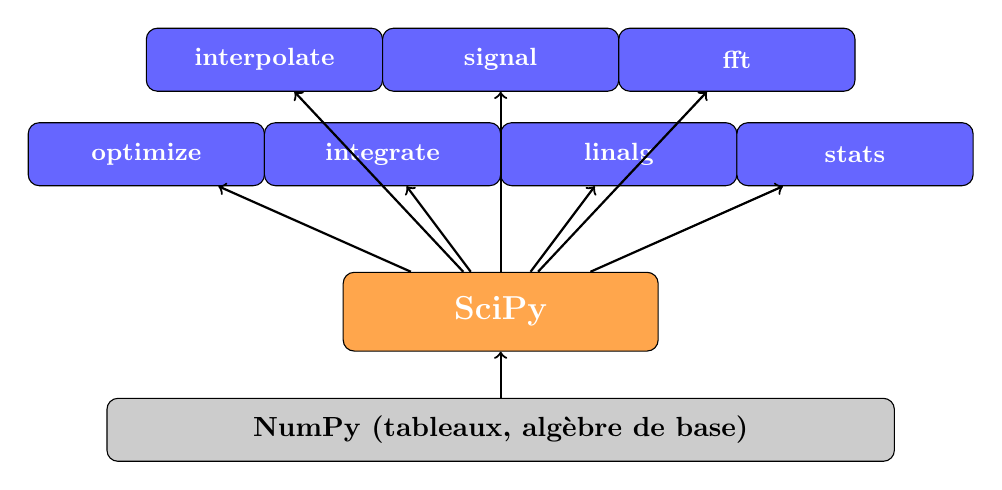
\begin{tikzpicture}[
  modbox/.style={draw, rounded corners, minimum width=3cm, minimum height=0.8cm,
                 fill=blue!60, text=white, font=\small\bfseries, align=center},
  corenode/.style={draw, rounded corners, minimum width=4cm, minimum height=1cm,
                   fill=orange!70, text=white, font=\large\bfseries, align=center},
  basenode/.style={draw, rounded corners, minimum width=10cm, minimum height=0.8cm,
                   fill=gray!40, font=\bfseries, align=center},
]
  % Base
  \node[basenode] (numpy) at (0,-3.5) {NumPy (tableaux, alg\`ebre de base)};

  % Core
  \node[corenode] (scipy) at (0,-2) {SciPy};

  % Modules
  \node[modbox] (opt) at (-4.5, 0) {optimize};
  \node[modbox] (int) at (-1.5, 0) {integrate};
  \node[modbox] (lin) at (1.5, 0)  {linalg};
  \node[modbox] (sta) at (4.5, 0)  {stats};
  \node[modbox] (interp) at (-3, 1.2) {interpolate};
  \node[modbox] (sig) at (0, 1.2)  {signal};
  \node[modbox] (fft) at (3, 1.2)  {fft};

  % Arrows
  \foreach \m in {opt, int, lin, sta, interp, sig, fft}
    \draw[->, thick] (scipy) -- (\m);
  \draw[->, thick] (numpy) -- (scipy);
\end{tikzpicture}
\end{center}

% ----------------------------------------------------------------
\section{\py{scipy.optimize} --- Optimisation et ajustement}
\index{scipy.optimize}\index{curve\_fit}\index{minimize}

\subsection{Ajuster une courbe exp\'erimentale avec \py{curve\_fit}}

En physique, on mesure souvent une d\'ecroissance exponentielle (radioactivit\'e,
d\'echarge d'un condensateur). Ajustons un mod\`ele $A(t) = A_0 \, e^{-\lambda t}$
\`a des donn\'ees bruit\'ees.

\begin{codeblock}[title=\textbf{Python}]
\begin{minted}{python}
import numpy as np
from scipy.optimize import curve_fit
import matplotlib.pyplot as plt

# Mod`ele exponentiel
def decroissance(t, A0, lam):
    return A0 * np.exp(-lam * t)

# Donn\'ees simul\'ees (avec bruit)
np.random.seed(42)
t_data = np.linspace(0, 10, 20)
y_data = 5.0 * np.exp(-0.3 * t_data) + 0.2 * np.random.randn(20)

# Ajustement
popt, pcov = curve_fit(decroissance, t_data, y_data)
A0_fit, lam_fit = popt
print(f"A0 = {A0_fit:.3f}, lambda = {lam_fit:.3f}")
\end{minted}
\end{codeblock}

\begin{codeoutput}
\begin{verbatim}
A0 = 5.047, lambda = 0.308
\end{verbatim}
\end{codeoutput}

Les valeurs retrouv\'ees ($A_0 \approx 5.05$, $\lambda \approx 0.31$) sont proches
des param\`etres r\'eels ($A_0 = 5$, $\lambda = 0.3$).

\begin{codeblock}[title=\textbf{Python}]
\begin{minted}{python}
# Visualisation
t_fine = np.linspace(0, 10, 200)
plt.scatter(t_data, y_data, label="Donn\'ees", color="black", s=20)
plt.plot(t_fine, decroissance(t_fine, *popt), "r-", label="Ajustement")
plt.xlabel("Temps (s)")
plt.ylabel("Activit\'e (Bq)")
plt.title("Ajustement d'une d\'ecroissance exponentielle")
plt.legend()
plt.show()
\end{minted}
\end{codeblock}

\subsection{Minimisation avec \py{minimize}}

\begin{codeblock}[title=\textbf{Python}]
\begin{minted}{python}
from scipy.optimize import minimize

# Trouver le minimum de f(x) = (x - 3)^2 + 2*sin(x)
def f(x):
    return (x - 3)**2 + 2 * np.sin(x)

result = minimize(f, x0=0)  # Point de d\'epart x0 = 0
print(f"Minimum en x = {result.x[0]:.4f}")
print(f"Valeur f(x) = {result.fun:.4f}")
\end{minted}
\end{codeblock}

\begin{codeoutput}
\begin{verbatim}
Minimum en x = 3.3424
Valeur f(x) = -1.8770
\end{verbatim}
\end{codeoutput}

% ----------------------------------------------------------------
\section{\py{scipy.integrate} --- Int\'egration num\'erique}
\index{scipy.integrate}\index{quad}

La fonction \py{quad}\index{quad} calcule une int\'egrale d\'efinie num\'eriquement.

\begin{definition}[Int\'egration num\'erique]
L'int\'egration num\'erique (ou quadrature) approxime la valeur d'une int\'egrale
d\'efinie $\int_a^b f(x)\,dx$ en \'evaluant $f$ en un nombre fini de points.
\end{definition}

\begin{codeblock}[title=\textbf{Python}]
\begin{minted}{python}
from scipy.integrate import quad

# Calculer l'int\'egrale de sin(x) de 0 `a pi
resultat, erreur = quad(np.sin, 0, np.pi)
print(f"Integrale de sin(x) de 0 a pi = {resultat:.6f}")
print(f"Valeur exacte = {2.0:.6f}")

# Int\'egrale gaussienne : int de -inf `a +inf de exp(-x^2)
val, err = quad(lambda x: np.exp(-x**2), -np.inf, np.inf)
print(f"Integrale gaussienne = {val:.6f}")
print(f"sqrt(pi) = {np.sqrt(np.pi):.6f}")
\end{minted}
\end{codeblock}

\begin{codeoutput}
\begin{verbatim}
Integrale de sin(x) de 0 a pi = 2.000000
Valeur exacte = 2.000000
Integrale gaussienne = 1.772454
sqrt(pi) = 1.772454
\end{verbatim}
\end{codeoutput}

% ----------------------------------------------------------------
\section{\py{scipy.linalg} --- Alg\`ebre lin\'eaire}
\index{scipy.linalg}\index{solve}\index{eig}

\subsection{R\'esoudre un syst\`eme lin\'eaire}

Consid\'erons le syst\`eme :
\[
\begin{cases}
2x + y = 5 \\
x + 3y = 7
\end{cases}
\quad \Longleftrightarrow \quad
\begin{pmatrix} 2 & 1 \\ 1 & 3 \end{pmatrix}
\begin{pmatrix} x \\ y \end{pmatrix}
=
\begin{pmatrix} 5 \\ 7 \end{pmatrix}
\]

\begin{codeblock}[title=\textbf{Python}]
\begin{minted}{python}
from scipy.linalg import solve, eig

A = np.array([[2, 1],
              [1, 3]])
b = np.array([5, 7])

x = solve(A, b)
print(f"Solution : x = {x[0]:.2f}, y = {x[1]:.2f}")
\end{minted}
\end{codeblock}

\begin{codeoutput}
\begin{verbatim}
Solution : x = 1.60, y = 1.80
\end{verbatim}
\end{codeoutput}

\subsection{Valeurs propres}

\begin{codeblock}[title=\textbf{Python}]
\begin{minted}{python}
# Valeurs propres et vecteurs propres
valeurs, vecteurs = eig(A)
print("Valeurs propres :", valeurs.real)
print("Vecteur propre 1 :", vecteurs[:, 0].real)
\end{minted}
\end{codeblock}

\begin{codeoutput}
\begin{verbatim}
Valeurs propres : [1.38196601 3.61803399]
Vecteur propre 1 : [-0.85065081  0.52573111]
\end{verbatim}
\end{codeoutput}

% ----------------------------------------------------------------
\section{\py{scipy.stats} --- Statistiques}
\index{scipy.stats}

\begin{codeblock}[title=\textbf{Python}]
\begin{minted}{python}
from scipy import stats

# G\'en\'erer des donn\'ees suivant une loi normale
np.random.seed(0)
echantillon = stats.norm.rvs(loc=170, scale=10, size=100)

# Statistiques descriptives
print(f"Moyenne : {np.mean(echantillon):.2f}")
print(f"Ecart-type : {np.std(echantillon, ddof=1):.2f}")

# Test de normalit\'e (Shapiro-Wilk)
stat, p = stats.shapiro(echantillon)
print(f"Test Shapiro-Wilk : p = {p:.4f}")
if p > 0.05:
    print("-> Distribution compatible avec la normalit\'e")
\end{minted}
\end{codeblock}

\begin{codeoutput}
\begin{verbatim}
Moyenne : 171.77
Ecart-type : 10.14
Test Shapiro-Wilk : p = 0.8453
-> Distribution compatible avec la normalite
\end{verbatim}
\end{codeoutput}

\begin{codeblock}[title=\textbf{Python}]
\begin{minted}{python}
# Test t de Student (deux \'echantillons)
groupe_a = stats.norm.rvs(loc=170, scale=10, size=50, random_state=1)
groupe_b = stats.norm.rvs(loc=175, scale=10, size=50, random_state=2)

t_stat, p_val = stats.ttest_ind(groupe_a, groupe_b)
print(f"t = {t_stat:.3f}, p-value = {p_val:.4f}")
\end{minted}
\end{codeblock}

\begin{codeoutput}
\begin{verbatim}
t = -2.574, p-value = 0.0116
\end{verbatim}
\end{codeoutput}

% ----------------------------------------------------------------
\section{\py{scipy.interpolate} --- Interpolation}
\index{scipy.interpolate}\index{interp1d}

L'interpolation permet d'estimer des valeurs entre des points de mesure.

\begin{codeblock}[title=\textbf{Python}]
\begin{minted}{python}
from scipy.interpolate import interp1d

# Points de mesure (temp\'erature en fonction du temps)
temps = np.array([0, 1, 2, 3, 4, 5])
temperature = np.array([20.0, 22.5, 28.3, 31.1, 29.0, 25.5])

# Interpolation lin\'eaire et cubique
f_lin = interp1d(temps, temperature, kind="linear")
f_cub = interp1d(temps, temperature, kind="cubic")

t_fin = np.linspace(0, 5, 100)
print(f"T `a t=2.5 (lin\'eaire) : {f_lin(2.5):.2f} °C")
print(f"T `a t=2.5 (cubique)  : {f_cub(2.5):.2f} °C")
\end{minted}
\end{codeblock}

\begin{codeoutput}
\begin{verbatim}
T a t=2.5 (lineaire) : 29.70 °C
T a t=2.5 (cubique)  : 30.22 °C
\end{verbatim}
\end{codeoutput}

\begin{codeblock}[title=\textbf{Python}]
\begin{minted}{python}
plt.scatter(temps, temperature, color="black", zorder=5,
            label="Mesures")
plt.plot(t_fin, f_lin(t_fin), "--", label="Lin\'eaire")
plt.plot(t_fin, f_cub(t_fin), "-", label="Cubique")
plt.xlabel("Temps (h)")
plt.ylabel("Temp\'erature (°C)")
plt.legend()
plt.title("Interpolation de donn\'ees de temp\'erature")
plt.show()
\end{minted}
\end{codeblock}

% ----------------------------------------------------------------
\begin{errmark}{Erreurs fr\'equentes avec SciPy}
\begin{enumerate}
  \item \textbf{Confondre \py{numpy.linalg} et \py{scipy.linalg}} ---
    Les deux existent, mais \py{scipy.linalg} est plus complet et plus optimis\'e.
    Pr\'ef\'erez toujours \py{scipy.linalg} pour les calculs s\'erieux.
  \item \textbf{Oublier le point de d\'epart dans \py{minimize}} ---
    La fonction \py{minimize} n\'ecessite un \py{x0}. Un mauvais choix initial peut
    conduire \`a un minimum \emph{local} au lieu du minimum global.
  \item \textbf{Mauvais mod\`ele dans \py{curve\_fit}} --- Si le mod\`ele math\'ematique
    ne correspond pas aux donn\'ees, l'ajustement sera mauvais. V\'erifiez toujours
    visuellement le r\'esultat.
  \item \textbf{Ignorer la matrice de covariance} --- \py{curve\_fit} retourne
    \'egalement \py{pcov}, qui permet de calculer les incertitudes sur les param\`etres
    ajust\'es : \py{np.sqrt(np.diag(pcov))}.
\end{enumerate}
\end{errmark}

% ----------------------------------------------------------------
\begin{projet}{Analyse et ajustement de donn\'ees exp\'erimentales}
Simulez une exp\'erience de d\'echarge d'un condensateur :
\begin{enumerate}
  \item G\'en\'erez des donn\'ees bruit\'ees suivant $V(t) = V_0 \, e^{-t/\tau}$
    avec $V_0 = 12$\,V et $\tau = 3$\,s (ajoutez du bruit gaussien).
  \item Utilisez \py{curve\_fit} pour retrouver $V_0$ et $\tau$.
  \item Calculez les incertitudes \`a partir de la matrice de covariance.
  \item Int\'egrez num\'eriquement l'\'energie dissip\'ee :
    $E = \int_0^{20} \frac{V(t)^2}{R}\,dt$ avec $R = 1\,\text{k}\Omega$.
  \item Tracez les donn\'ees, la courbe ajust\'ee et les barres d'erreur.
  \item Comparez le $\tau$ obtenu avec la valeur th\'eorique.
\end{enumerate}
\end{projet}

% ----------------------------------------------------------------
\section{Exercices}

\begin{exercice}[$\star$]
Calculez num\'eriquement l'int\'egrale $\displaystyle\int_0^1 e^{-x^2}\,dx$ avec
\py{quad}. Comparez avec la valeur approch\'ee $\approx 0.7468$.
\end{exercice}

\begin{exercice}[$\star$]
R\'esolvez le syst\`eme lin\'eaire :
$3x + 2y - z = 1$, $2x - y + 4z = -2$, $x + y + z = 0$.
V\'erifiez en calculant $A \cdot x$ avec NumPy.
\end{exercice}

\begin{exercice}[$\star\star$]
G\'en\'erez 200 points suivant une loi normale ($\mu = 50$, $\sigma = 8$).
Effectuez un test de Shapiro-Wilk et un test de Kolmogorov-Smirnov
(\py{stats.kstest}) pour v\'erifier la normalit\'e. Interpr\'etez les p-valeurs.
\end{exercice}

\begin{exercice}[$\star\star$]
Des donn\'ees exp\'erimentales suivent la loi $y = a \sin(bx + c)$.
G\'en\'erez des donn\'ees avec $a=3$, $b=2$, $c=0.5$ plus du bruit.
Utilisez \py{curve\_fit} pour retrouver les param\`etres. Attention : donnez
des valeurs initiales raisonnables avec le param\`etre \py{p0}.
\end{exercice}

\begin{exercice}[$\star\star\star$]
Mod\'elisez la cin\'etique d'une r\'eaction chimique du second ordre :
$\frac{d[A]}{dt} = -k[A]^2$. La solution analytique est
$[A](t) = \frac{[A]_0}{1 + k[A]_0 t}$. G\'en\'erez des donn\'ees bruit\'ees,
ajustez le mod\`ele pour trouver $k$ et $[A]_0$, puis int\'egrez num\'eriquement
$\int_0^{10} [A](t)\,dt$ (quantit\'e totale restante). Comparez int\'egration
num\'erique et solution analytique.
\end{exercice}

% ----------------------------------------------------------------
\begin{formules}{Chapitre 10 --- SciPy : l'essentiel}
\begin{tabular}{@{}p{4.5cm} p{9.5cm}@{}}
\toprule
\textbf{Sous-module} & \textbf{Fonctions cl\'es} \\
\midrule
\py{scipy.optimize} & \py{minimize(f, x0)}, \py{curve\_fit(modele, x, y)} \\
\py{scipy.integrate} & \py{quad(f, a, b)} --- int\'egrale d\'efinie \\
\py{scipy.linalg} & \py{solve(A, b)}, \py{eig(A)} \\
\py{scipy.stats} & \py{ttest\_ind}, \py{shapiro}, distributions \\
\py{scipy.interpolate} & \py{interp1d(x, y, kind="cubic")} \\
\midrule
\multicolumn{2}{@{}l}{\textbf{Astuces}} \\
\midrule
Incertitudes fit & \py{np.sqrt(np.diag(pcov))} \\
Bornes infinies & \py{quad(f, -np.inf, np.inf)} \\
Valeurs initiales & \py{curve\_fit(f, x, y, p0=[a0, b0])} \\
\bottomrule
\end{tabular}
\end{formules}
